\documentclass[a4paper,12pt]{article}
\usepackage[english,vietnamese]{babel}
\usepackage{amsmath}
\usepackage{booktabs}
\usepackage{lmodern}
\usepackage[utf8]{inputenc}
\usepackage{graphicx}
\usepackage{hyperref}
\usepackage{lmodern}
\usepackage[nottoc,numbib]{tocbibind}
\newcommand{\id}[1]{\underline{#1\_id}}
\renewcommand{\thefootnote}{\fnsymbol{footnote}}

\begin{document}
\setcounter{page}{0}
\thispagestyle{empty}
\vspace*{\stretch{1}}
\begin{flushright}
  \setlength{\baselineskip}{1.4\baselineskip}
\textbf{\Huge Python Package\\Metadata Management}
  \noindent\rule{\textwidth}{5pt}
  \emph{\Large Basic Databases}
  \vspace{\stretch{1}}

  \textbf{by Nguyễn Gia Phong, Nguyễn Quốc Thông,\\
          Nguyễn Văn Tùng and Trần Minh Vương\\}
  \selectlanguage{english}
  \today
\end{flushright}
\vspace*{\stretch{2}}
\pagebreak

\selectlanguage{english}
\tableofcontents
\pagebreak

\section{Introduction}
\subsection{Brief Description}
In traditional Unix-like operating systems like GNU/Linux distributions
and BSD-based OSes, package managers tries to synchronize the packages metadata
(such as available versions and dependencies) with that of central repositories.
While this proves to be reliable and efficient, language-specific
package managers do not usually have such synchronized databases,
since they focus on development libraries which have more flexible contraints.

Within the Python packaging ecosystem, this is the case, where package managers
like \verb|pip| needs to fetch metadata of each package to be installed
to find out dependencies and other information.  This turns out to have heavy
performance penalty on the dependency resolution process alone, which is
already a NP-hard problem.  This project explores ways to store these metadata
in an efficient in a database, to be used in practice either locally or in a
local/regional network, to avoid Python package managers from having to
fetch (and potentially build) entire packages just to find out if it conflicts
with others.

\selectlanguage{vietnamese}
\subsection{Authors and Credits}
The work has been undertaken by group number 8, whose members are listed
in the following table.
\begin{center}
  \begin{tabular}{c c}
    \toprule
    Full name & Student ID\\
    \midrule
    Nguyễn Gia Phong & BI9-184\\
    Nguyễn Quốc Thông & BI9-214\\
    Nguyễn Văn Tùng & BI9-229\\
    Trần Minh Vương & BI9-239\\
    \bottomrule
  \end{tabular}
\end{center}

This report is licensed under a CC BY-SA 4.0 license, while the source code is
available on GitHub\footnote{\url{https://github.com/McSinyx/cheese-shop}}
under AGPLv3+.

We would like to express our special thanks to Dr. Nguyễn Hoàng Hà,
whose lectures gave us basic understanding on the key principles of
relational databases.  In addition, we also recieved a lot of help from
the Python packaging community over \#pypa on Freenode on understanding
the structure of the metadata as well as finding a way to fetch these
data from package indices.

\selectlanguage{english}
\section{User Requirements}
This project aims to provide a database for metadata queries and Python packages
exploration.  We try to replicate the PyPI's XML-RPC API~\cite{xmlrpc},
which supports queris similar to the following:
\begin{itemize}
  \item \verb|list_projects()|: Retrieve a list of registered project names.
  \item \verb|project_releases(project)|: Retrieve a list of releases for
    the given \verb|project|, ordered by version.
  \item \verb|project_release_latest()|: Retrieve the latest release
    of the given \verb|project|.
  \item \verb|belong_to(name)|: Retrieve a list of projects whose author
    is \verb|name|.
  \item \verb|browse(classifier)|: Retrieve a list of (\verb|project|,
    \verb|version|) of all releases classified with all of the given classifier.
  \item \verb|release_data(project, version)|: Retrieve the following metadata
    matching the given release: project, version, homepage, author,
    author's email, summary, license, keywords, classifiers and dependencies
  \item \verb|search_name(pattern)|: Retrieve a list of (\verb|project|,
    \verb|version|, \verb|summary|) where the project name matches the pattern.
  \item \verb|search_summary(pattern)|: Retrieve a list of (\verb|project|,
    \verb|version|, \verb|summary|) where the summary matches the pattern.
\end{itemize}

\section{Data Definition}
\subsection{Entity Relationship Diagram}
The entity relationship diagram represents the relationship between each of
its entity set of data extracted from projects:
\begin{itemize}
  \item Author(Releases-Contact: Many-One): Within each release, there could be
    one author, due to data extraction method doesn't support multi-author.
    Yet an author could have multiple releases under per name.
  \item Require(Releases-Dependencies: Many-Many): Every release would require
    a number of dependencies, and many dependencies can each be used by
    multiple releases.
  \item Classify(Releases-Trove: Many-Many): This relationship indicates the
    relationship between trove classifier and each releases, with many release
    could be classified under one trove classifier, and a release could be
    classified by many classifiers.
  \item Contain(Releases-Keyword: Many-Many): A release has many keywords,
    and also a keyword can also be in many different releases.
  \item Release(Releases-Distribution: One-Many): Within each releases,
    a number of distribution(s) would be released.  A distribution could
    relate to only one releases, but many distributions could be released
    in the same releases.
\end{itemize}
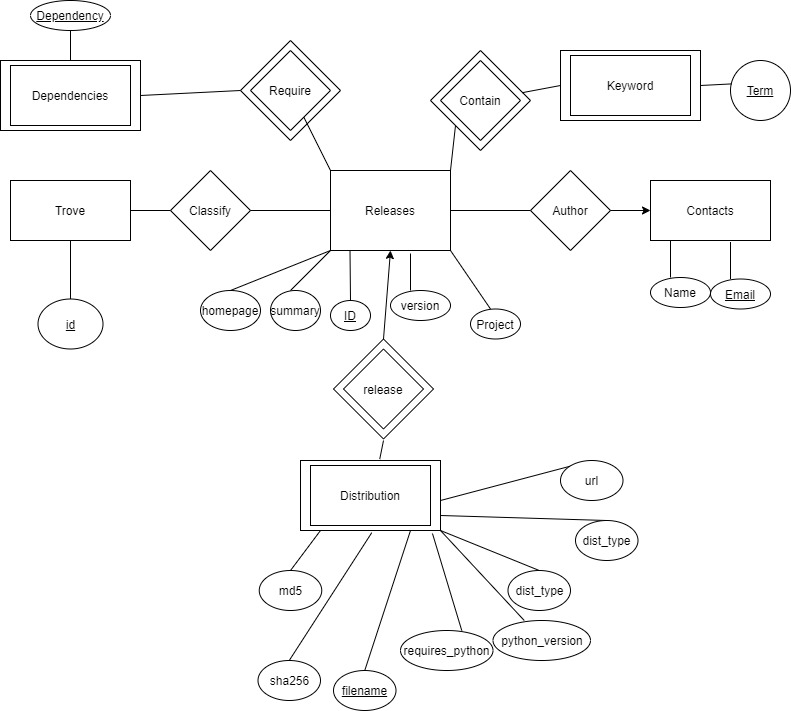
\includegraphics[width=\textwidth]{erd.jpg}

\subsection{Database Schema}
Based on the entity relationship diagram, we worked out a schema complying
with the third normal form~\cite{3nf}.
\begin{center}
  \includegraphics[width=\textwidth]{schema.png}
\end{center}

\paragraph{contacts(\underline{email}, name)} Contact information of an author,
including per email as the primary key and per name.

\paragraph{releases(\underline{id}, project, version, summary, homepage, email)}
This relation represents each release of a project, including its name, version,
summary, homepage and the email of its author.  The ID of each release is
the primary key to represent each one of them.  This release ID is also
the foreign key of many primary key in other entity set.

\paragraph{troves(\underline{id}, classifier)} Valid trove classifiers,
identified by their ID.

\paragraph{classifiers(\id{release}, \id{trove})}
Release ID and corresponding trove classifiers ID the release is classified by.

\paragraph{keywords(\id{release}, \underline{term})} Keywords of a specific
release.  Both the ID of the release and the keyword are set as primary key.

\paragraph{dependencies(\id{release}, \underline{dependency})} This relation
represents the dependency list of each release, which is a pattern can be
matched by a release of another project.

\paragraph{distributions(\id{release}, \underline{filename}, size, url,
dist\_type, python\_version, requires\_python, sha256, md5)}
Each distribution (i.e. the file that the package manager can use to install)
and the corresponding url, checksums and other auxiliary information.

\section{Data Query}
\subsection{Project Listing}
Retrieve a list of registered project names
\begin{verbatim}
SELECT DISTINCT project FROM releases
\end{verbatim}

\subsection{Project Releases}
Retrieve a list of releases for the given project name, ordered by version.
\begin{verbatim}
SELECT * FROM releases
WHERE project = 'numpy'
ORDER BY version
\end{verbatim}

\subsection{Project Latest Release}
Retrieve the latest version of the given project.
\begin{verbatim}
SELECT *
FROM releases
WHERE project = 'numpy'
ORDER BY version
LIMIT 1
\end{verbatim}

\subsection{User's Project}
Retrieve a list of projects whose author is name.
\begin{verbatim}
SELECT project
FROM releases
LEFT JOIN contacts
ON releases.email = contacts.email
WHERE contacts.name = 'Travis E. Oliphant et al.'
\end{verbatim}

\subsection{Classifiers}
Retrieve a list of name, version of all releases classified with all the given classifiers, classifiers must be a list of Trove classifier strings.
\begin{verbatim}
SELECT releases.name, releases.version, troves.classifier
FROM releases
JOIN classifier ON releases.id = classifier.release_id
INNER JOIN troves ON classifier.trove_id = troves.id
WHERE troves.classifier = 'Python'
\end{verbatim}

\subsection{Release Data}
Retrieve metadata describing a specific release.
\begin{verbatim}
SELECT rls.project, rls.version, rls.homepage, rls.author,
       rls.email, rls.summary, keywords.term,
       classiffier.troves.classifier,
       dependencies.dependency
FROM releases AS rls
INNER JOIN contacts ON rls.email = contacts.email
RIGHT JOIN (classifier
            INNER JOIN troves
            ON classifier.trove_id = troves.id)
      ON rls.id = classifier.release_id
RIGHT JOIN keywords ON rls.id = keywords.release_id
RIGHT JOIN dependencies ON rls.id = dependencies.release_id
WHERE rls.id = '1'
\end{verbatim}

\subsection{Search project by name}
Retrieve project by name SQL pattern
\begin{verbatim}
SELECT project, version, summary
FROM releases
WHERE project LIKE 'py%'
\end{verbatim}

\subsection{Search project name by summary}
Retrieve project by summary SQL pattern
\begin{verbatim}
SELECT project, version, summary
FROM releases
WHERE summary LIKE '%num%'
\end{verbatim}

\section{Conclusion}

\begin{thebibliography}{69}
  \bibitem{xmlrpc} The Python Packaging Authority.
    \href{https://warehouse.readthedocs.io/api-reference/xml-rpc}
         {\emph{PyPI’s XML-RPC methods}}.
    Warehouse documentation.
  \bibitem{3nf} Edgar~F.~Codd.
    \emph{Further Normalization of the Data Base Relational Model}.
    IBM Research Report RJ909, August 31, 1971.
\end{thebibliography}
\end{document}
